\section{Конструкторский раздел}
В этом разделе будет проведено проектирование базы данных и приложения.
Будут приведены созданные таблицы, поля таблиц с указанием их семантического смысла.
Будет представлена ER-модель созданной базы данных.
Будет разработана UML-диаграмма разрабатываемого приложения.
Будет выбран тип приложения.
Будут представлены схемы основных алгоритмов, необходимых для функционирования букмекерской конторы.

\subsection{Проектирование базы данных}
База данных приложения будет реализована с помощью следующих страниц:
\begin{enumerate}
	\item таблица пользователей User;
	\item таблица игроков Account;
	\item таблица команд Teams;
	\item таблица матчей Games;
	\item таблица ставок Bet;
\end{enumerate}

Таблица пользователей \textbf{User} содержит информацию о логинах, паролях аккаунтов, а также о ролях, соответствующих аккаунту.
Содержит следующие поля:
\begin{itemize}
	\item id -- первичный ключ, идентификатор аккаунта;
	\item userLogin -- логин пользователя;
	\item password -- пароль пользователя;
	\item creationDate -- дата регистрации аккаунта;
	\item userRole -- роль, соответствующая аккаунту.
\end{itemize}

Таблица пользователей \textbf{Account} содержит информацию о личности игрока, который совершает ставки в букмекерской конторе.
Содержит следующие поля:
\begin{itemize}
	\item accID -- первичный ключ, идентификатор аккаунта;
	\item userID -- внешний ключ, соответствует идентификаторам интернет аккаунта;
	\item userName -- имя пользователя, указанное при регистрации;
	\item userSurname -- фамилия пользователя, указанное при регистрации;
	\item dateOfBirth -- дата рождения пользователя;
	\item phoneNumber -- номер телефона пользователя;
	\item email -- электронная почта пользователя;
	\item passportNumber -- номер паспорта пользователя;
	\item userStatus -- статус пользователя: на верификации, активный и заблокированный аккаунты;
	\item balance -- текущий баланс пользователя;
	\item maxBet -- размер максимальной ставки, доступной игроку.
\end{itemize}

Таблица команд \textbf{Teams} содержит информацию о командах, которые могут принимать участие в матче.
Содержит следующие поля:
\begin{itemize}
	\item teamID -- первичный ключ, идентификатор команды;
	\item teamName -- название команды;
	\item teamcity -- город, из которого команда;
	\item logo -- локальный путь к картинке эмблемы команды.
\end{itemize}

Таблица матчей \textbf{Games} содержит информацию о матчах, на которые принимаются ставки в букмекерской конторе.
Содержит следующие поля:
\begin{itemize}
	\item gameID -- первичный ключ, идентификатор матча;
	\item gameStatus -- соответствует текущему состоянию матча: запланирован, идёт или закончился;
	\item team1ID -- внешний ключ, соответствует id первой команды;
	\item team2ID -- внешний ключ, соответствует id второй команды;
	\item w1Coef -- текущий коэффициент на победу первой команды;
	\item drawCoef -- текущий коэффициент на ничью;
	\item w2Coef -- текущий коэффициент на победу второй команды;
	\item gameResult -- текущий счёт в матче;
	\item gameDate -- дата проведения матча;
	\item gameTime -- время начала матча;
\end{itemize}

Таблица ставок \textbf{Bet} содержит информацию о совершённых пользователями ставках.
Содержит следующие поля:
\begin{itemize}
	\item betID -- первичный ключ, идентификатор ставки;
	\item gameID -- внешний ключ, соответствует идентификатору матча;
	\item accID -- внешний ключ, соответствует id пользователя, который совершил ставку;
	\item choosedResult -- выбранный результат (0 -- ничья, 1 -- победа первой команды, 2 -- победа второй команды);
	\item betDate -- время совершения ставки;
	\item betSize -- размер совершенной ставки;
	\item koef -- коэффициент, по которому игрок совершил ставку;
	\item betStatus -- текущее состояние ставки: принята, выиграна или проиграна;
	\item payoutAmount -- выплата по результатам совершения события;
\end{itemize}

\newpage

ER-модель БД в нотации Crow’s Foot представлена на рисунке 3:
\FloatBarrier
\begin{figure}[h]	
	\begin{center}
		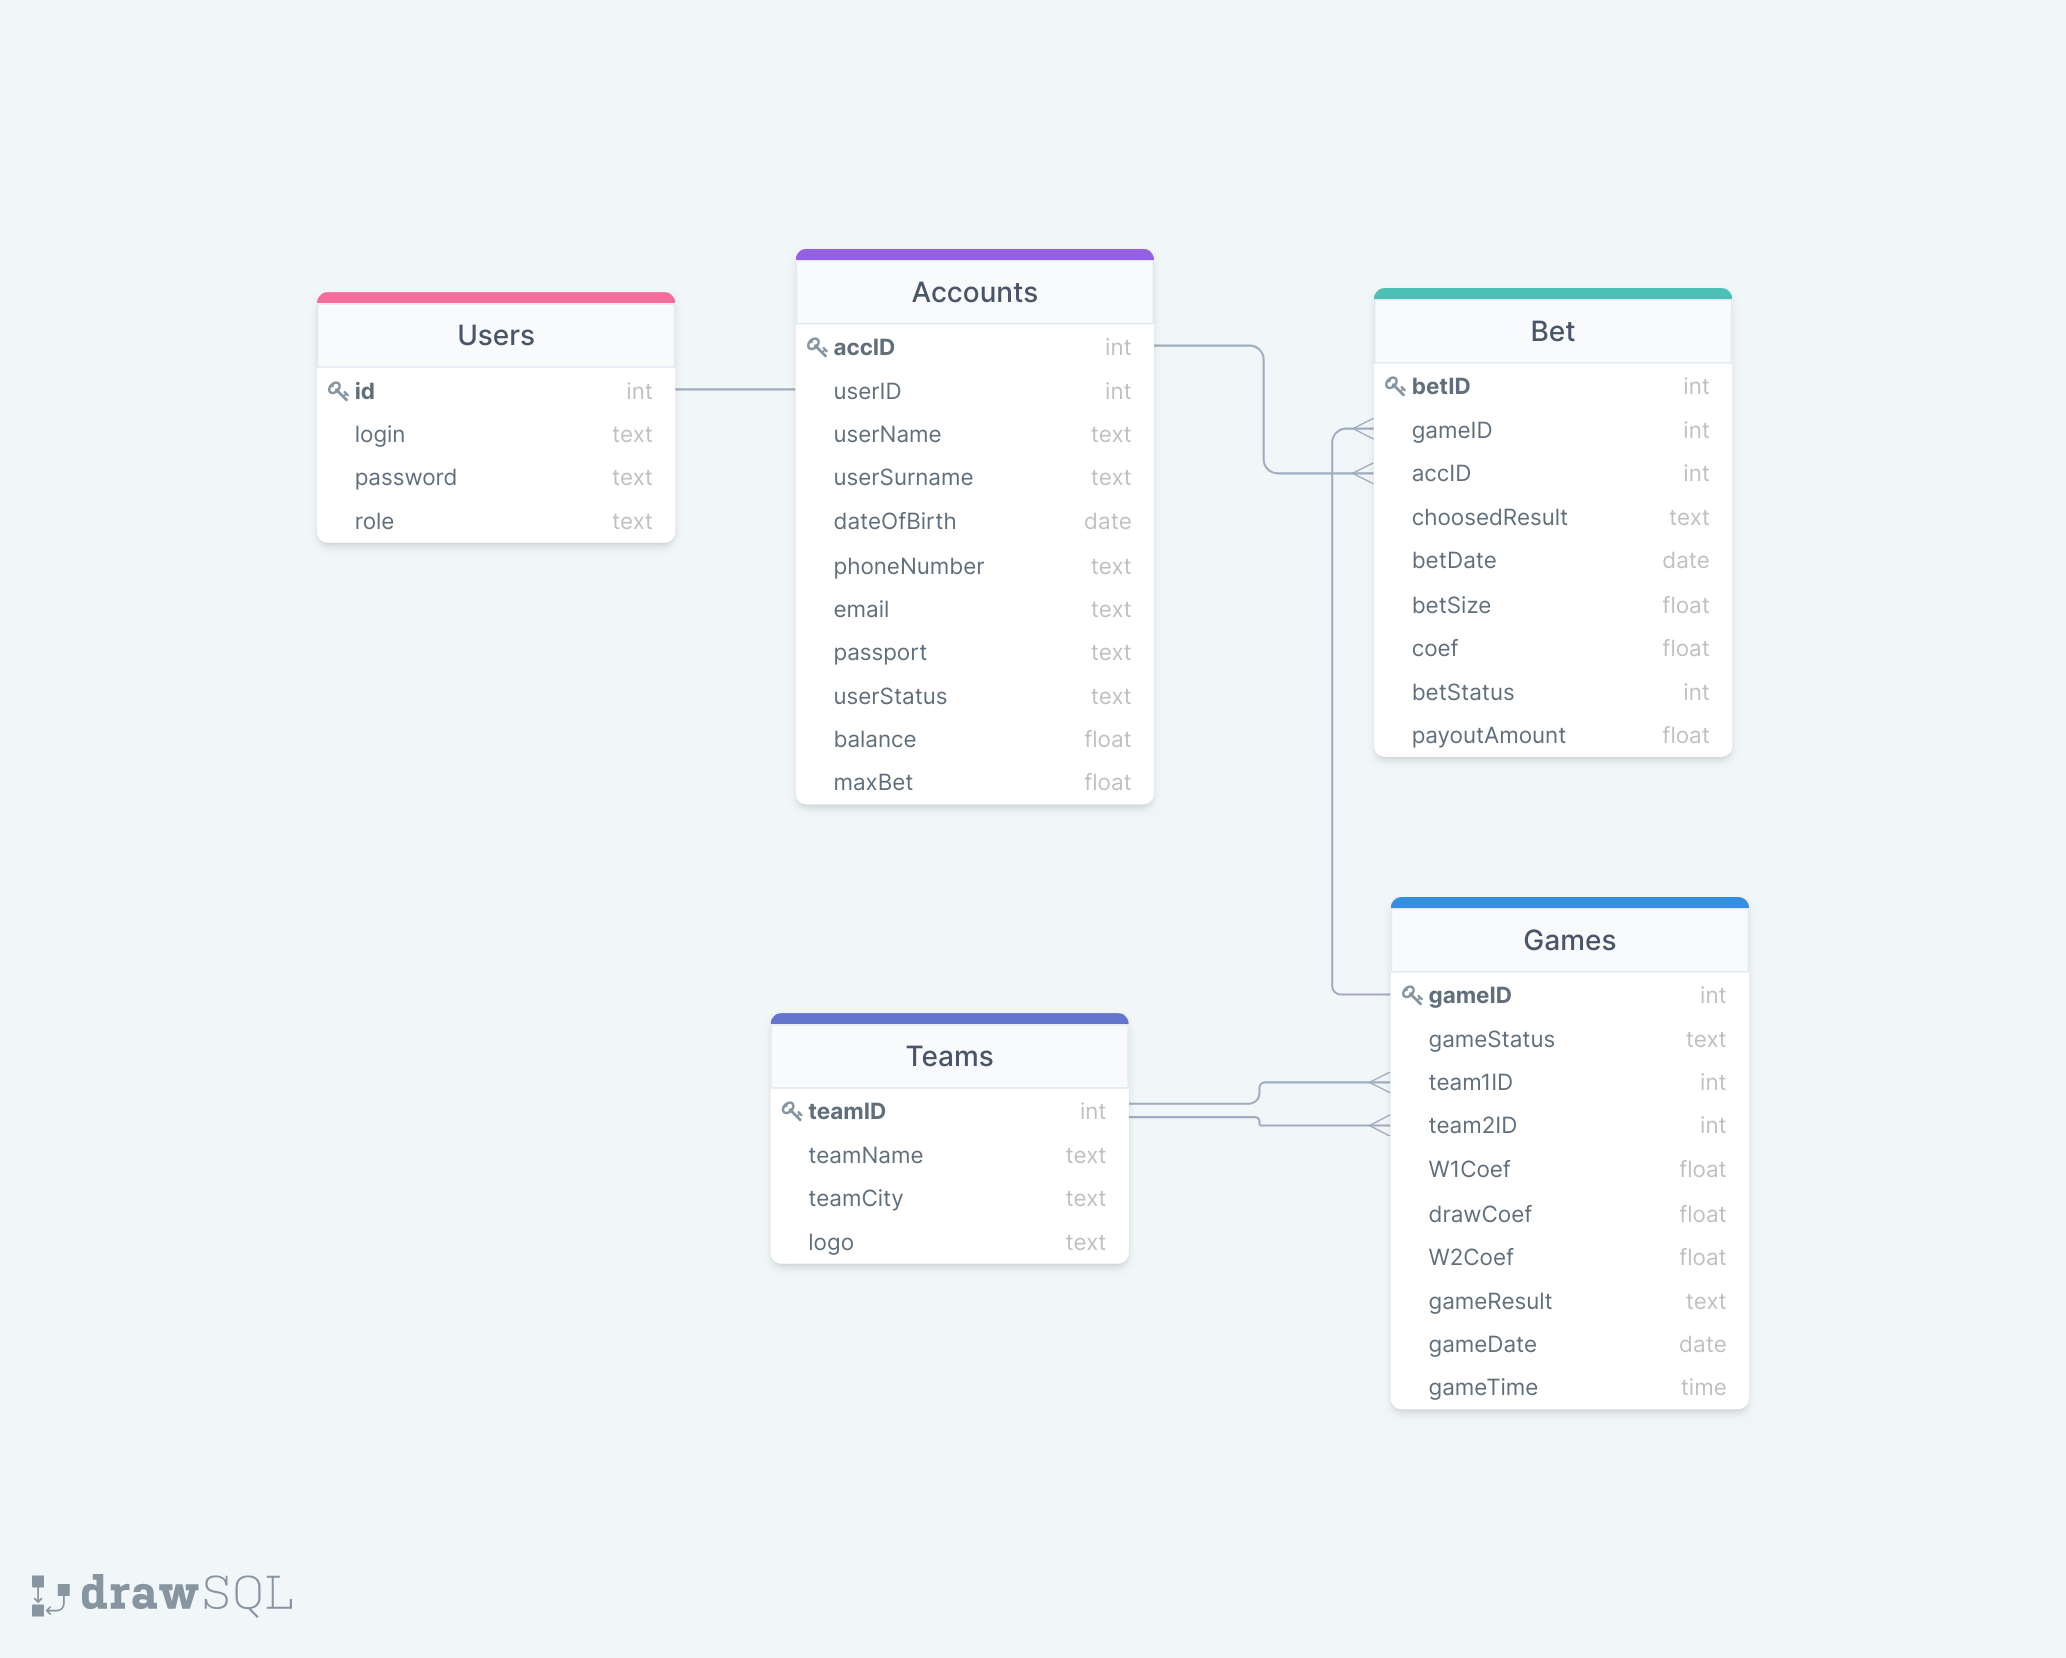
\includegraphics[width=\linewidth]{inc/scheme.png}
	\end{center}
	\captionsetup{justification=centering, labelsep=defffis}
	\caption{ER-модель базы данных в нотации Crow’s Foot}
	\label{fig::scheme}
\end{figure}
\FloatBarrier

\subsection{Тип приложения}
Тип приложения был выбран Desktop по двум следующим причинам:
\begin{enumerate}
	\item Реальные букмекерские конторы разрабатывают версии программного обеспечения для ПК, так как это позволяет пользователям удобнее и быстрее взаимодействовать с системой.
	\item Desktop-приложение не предоставляет дополнительных требований к времени ответу системы, как, например, высоконагруженный сервис. 
	\item Автор имеет опыт разработки Desktop приложений.
\end{enumerate}

Выбранный тип приложения позволяет перейти к непосредственно её проектированию.
\subsection{Проектирование приложения}
Структура приложения основана на парадигмах ООП. 

Для реализации работы приложения были реализованы следующие классы:
\begin{itemize}
	\item class UI -- класс содержит функции для загрузки новой страницы формата .ui и создания контроллера под неё;
	\item class Controllers -- набор классов, каждый из которых контролирует связь элементов страниц друг с другом;
	\item class Facade -- класс, является реализацией паттерна «Фасад»;
	\item class Command -- набор классов, являются реализацией паттерна «Команда»;
	\item class AuthManager -- класс, являющийся сущностью между действий в UI и базой данных для неавторизованного пользователя;
	\item class PlayerManager -- класс, являющийся сущностью между действий в UI и базой данных для вошедшего в систему игрока;
	\item class AdminManager -- класс, являющийся сущностью между действий в UI и базой данных для администратора БК;
	\item class AnalyzerManager -- класс, являющийся сущностью между действий в UI и базой данных для аналитика;
	\item class AuthRepo -- класс, непосредственно взаимодействующий с базой данных для неавторизованного пользователя; 
	\item class PlayerRepo -- класс, непосредственно взаимодействующий с базой данных для авторизованного игрока; 
	\item class AdminRepo -- класс, непосредственно взаимодействующий с базой данных для администратора БК; 
	\item class AnalyzerRepo -- класс, непосредственно взаимодействующий с базой данных для аналитика; 
	\item class SessionHolder -- класс, реализующий паттерн «Прокси», выполняющий хэширование данных текущего игрока. Позволяет не взаимодействовать с БД для получения данных пользователя;
	\item class ValidateManager -- набор классов, валидующих данные: при регистрации, при добавлении нового матча или корректировке коэффициентов.
\end{itemize}

На рисунке 4 представлена UML-диаграмма классов.
\FloatBarrier
\begin{figure}[h]	
	\begin{center}
		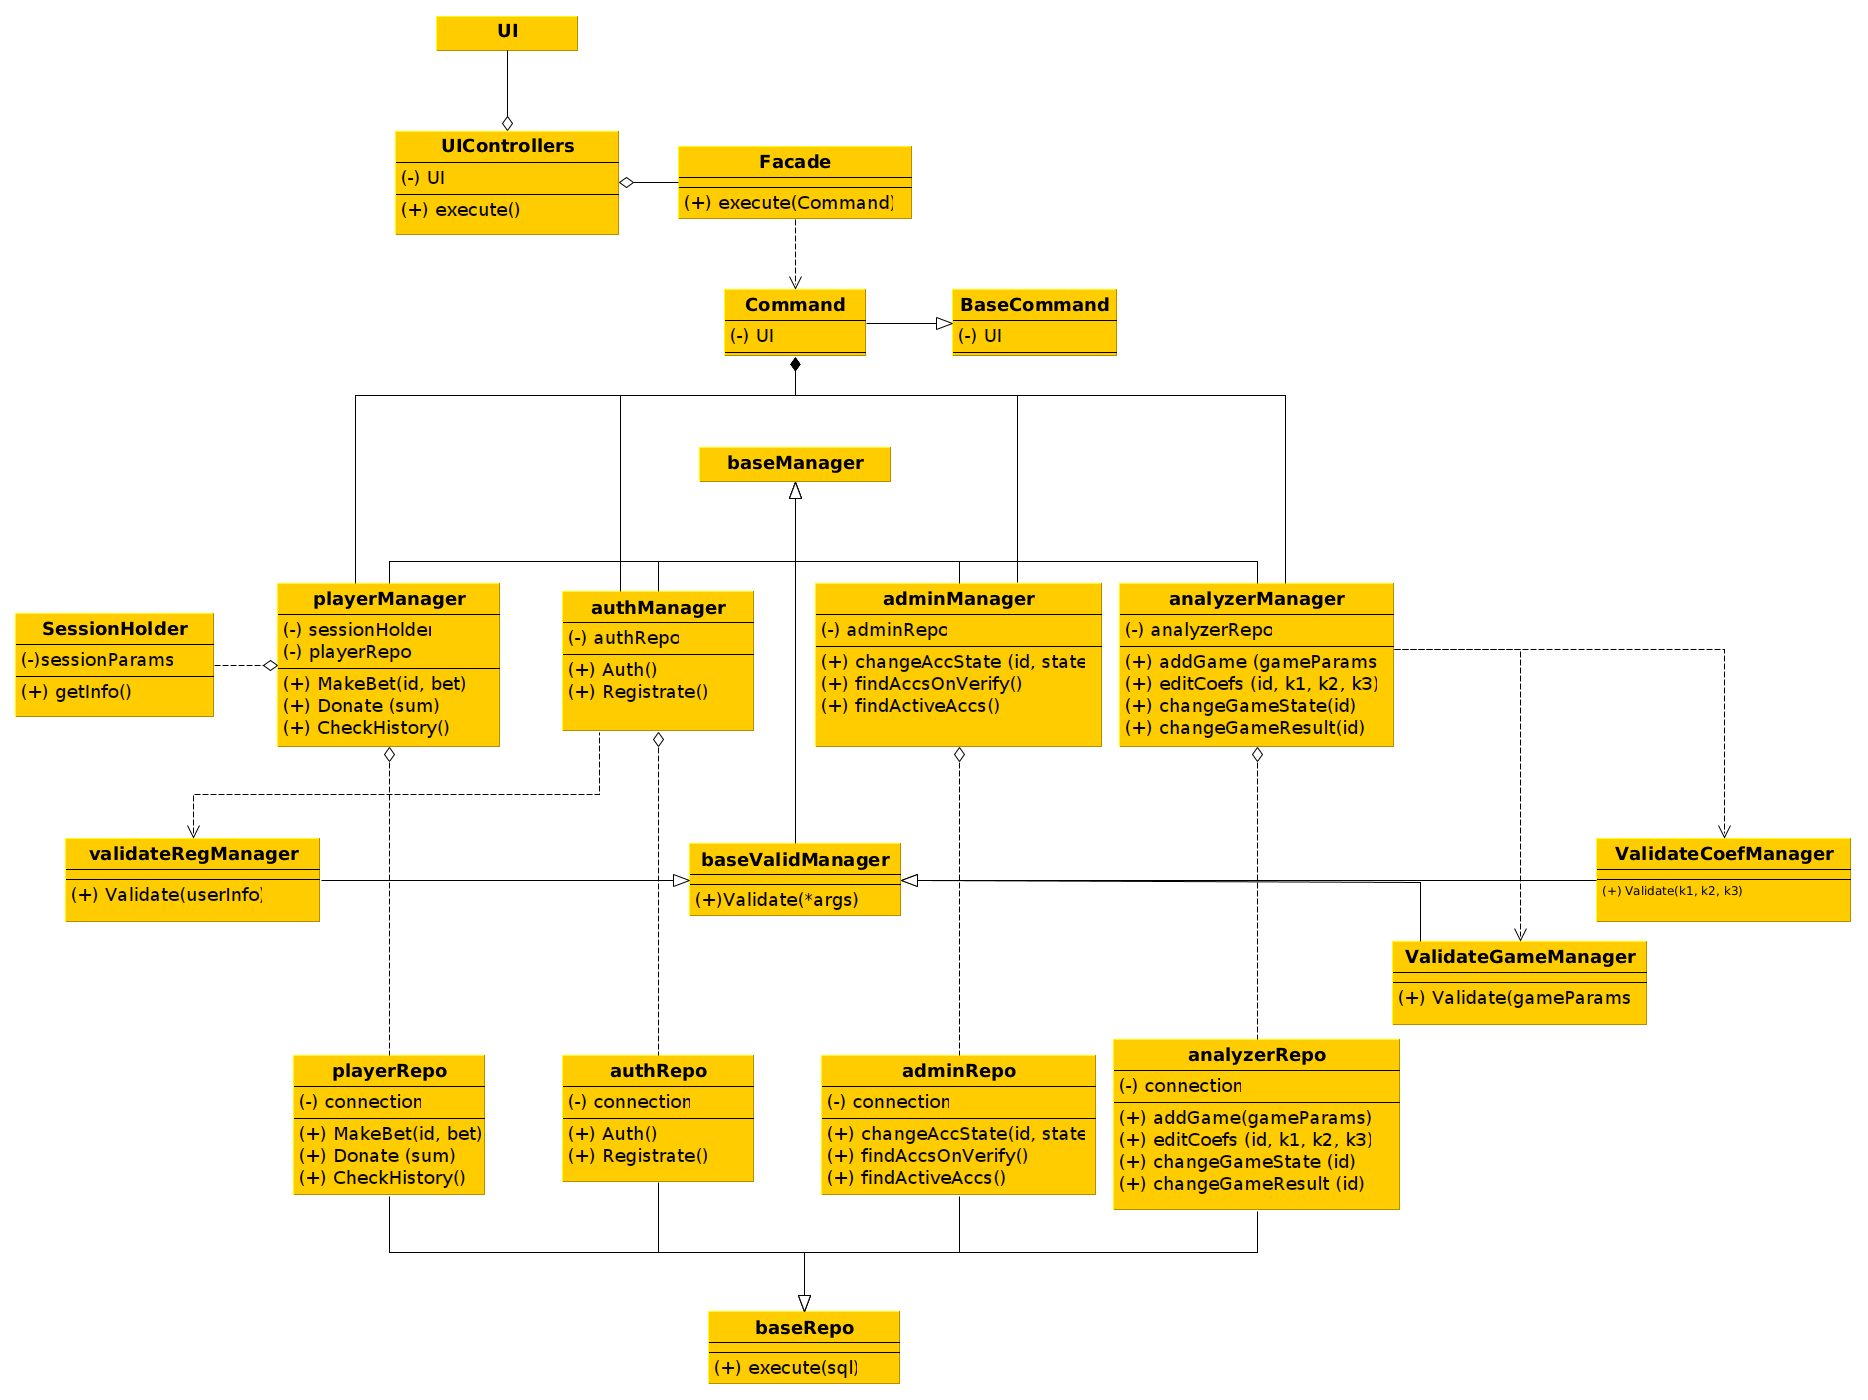
\includegraphics[angle=90, width=\linewidth, height=16cm]{inc/uml.png}
	\end{center}
	\captionsetup{justification=centering, labelsep=defffis}
	\caption{UML-диаграмма классов}
	\label{fig::uml}
\end{figure}
\FloatBarrier

\subsection{Алгоритм работы программы при авторизации пользователя}
Авторизация пользователя происходит при активном взаимодействии с базой данных.

В первую очередь требуется проверить, что логин существует в базе данных. 
Для этого достаточно найти одно значение логина в базе, при этом гарантируется, что поле логина уникальное, и логин присутствует в единственном экземпляре.

После соответствия требуется проверить соответствие введенного пароля и пароля в системе. 
Если они совпадают, то можно выполнить вход в систему, иначе вывести сообщение об ошибке.

При входе системе требуется также получить из БД роль, соответствующую аккаунту, в который входит пользователь.
Для аналитика и администратора в дальнейшем загружается UI, но для игрока требуется провести несколько дополнительных действий.

Во-первых, требуется выгрузить из БД всю основную информацию о пользователе, и кэшировать её.
Это нужно для того, чтобы в дальнейшем не обращаться к БД для проверки параметров (например, хватает ли у пользователя средств для совершения ставки), что снижает время работы с самой базой данных.
Во-вторых, требуется проверить, какой статус у аккаунта. 
Если у пользователя заблокированный аккаунт, то он не может выполнять никаких действий, поэтому требуется в UI заблокировать все соответствующие элементы.

\newpage
На рисунке 5 представлена схема алгоритма работы программы при авторизации:
\FloatBarrier
\begin{figure}[h]	
	\begin{center}
		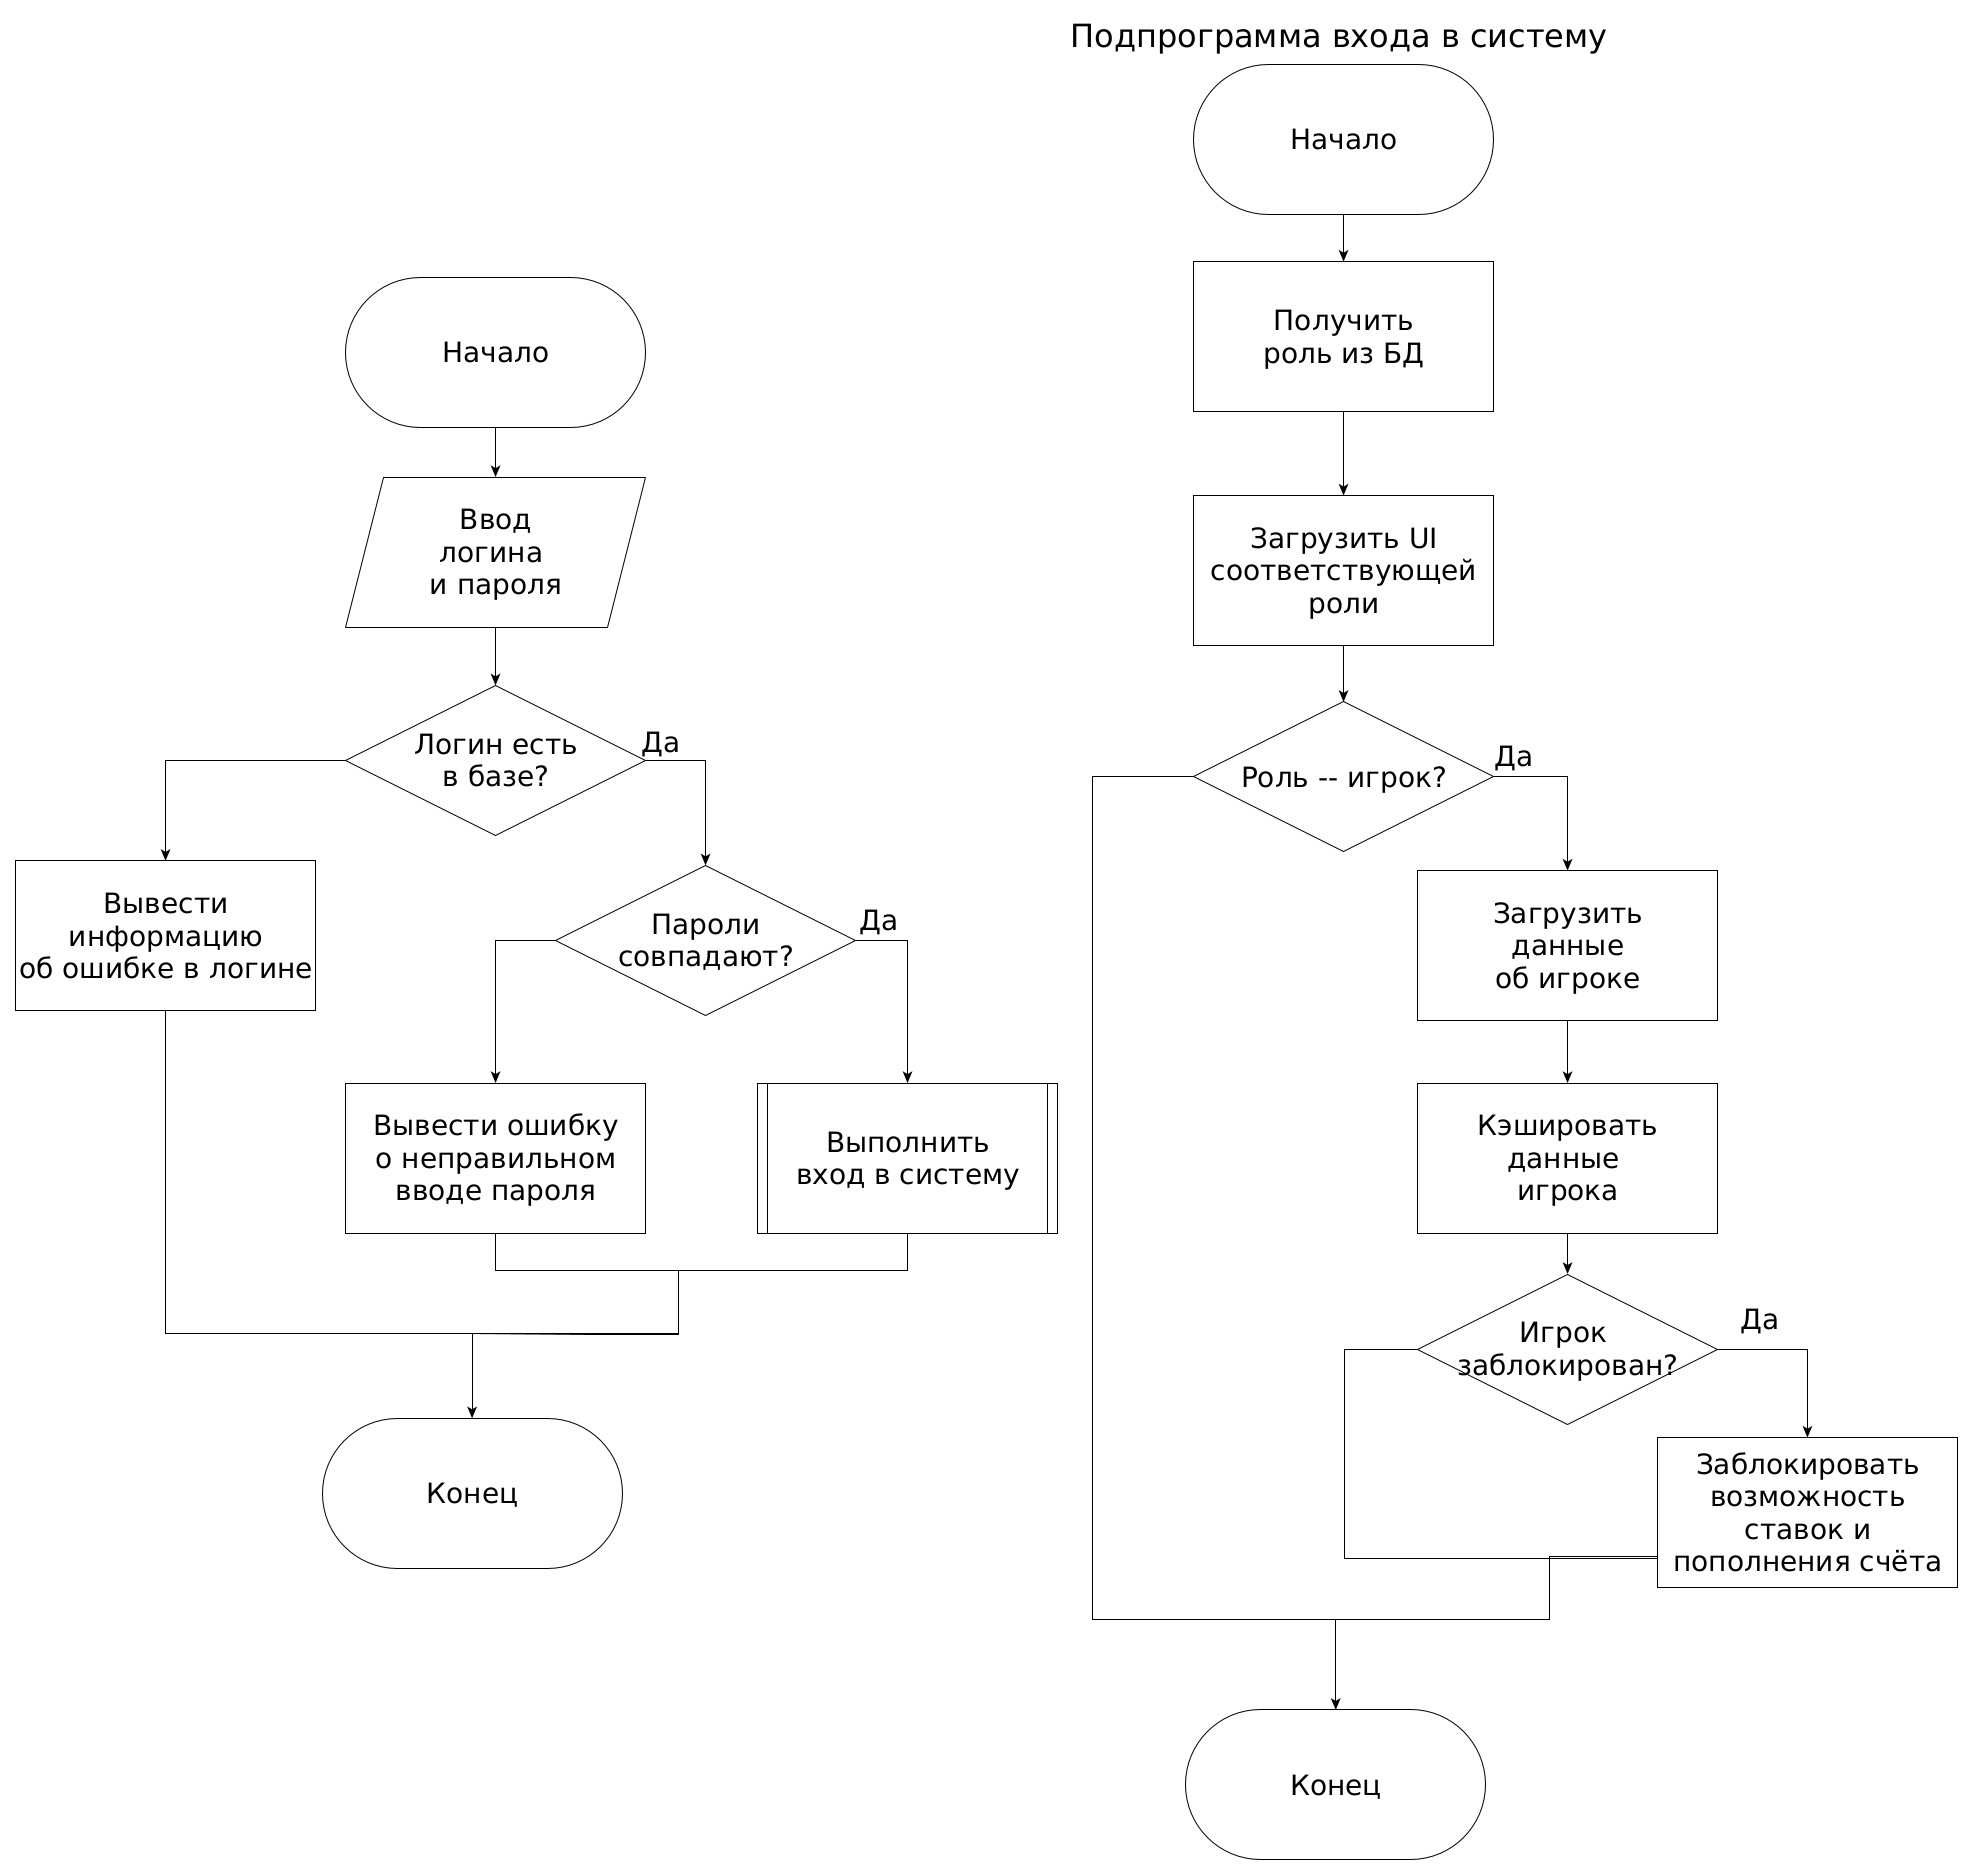
\includegraphics[width=\linewidth]{inc/auth.png}
	\end{center}
	\captionsetup{justification=centering, labelsep=defffis}
	\caption{Схема алгоритма работы программы при авторизации}
	\label{fig::auth}
\end{figure}
\FloatBarrier

\newpage
\subsection{Алгоритм работы при обновлении состояния матча}
Алгоритм работы при обновлении состояния матча является важнейшим для работы системы, так как расчёт выплат по ставкам производится по окончанию матча.

Для автоматического обновления баланса пользователей требуется разработать триггер.
Он будет навешан на таблицу Bet, но сложность заключается в том, что баланс находится в другом отношении -- Account.
Следовательно, требуется вызывать подпрограмму для обновления баланса пользователей.

Также для определения результата матча требуется реализовать собственную функцию, так как в таблице хранится текущий счёт встречи: в таблице нельзя отдельно хранить результат из-за того, что тогда возникнет избыточность в базе, а счёт требуется для корректной оценки пользователем действий в матче. 

Для обновления статуса ставок требуется сравнить результат, выбранный игроком, и реальный. 
Статус ставки хранится в виде целочисленного флага: 1 соответствует выигрышу, 0 -- проигрышу.

Для последовательного прохода по id требуется реализовать курсор, так как требуется изменять баланс пользователей построчно, последовательно итерируясь по всем пользователям, делавших ставки на конкретное событие.

\newpage
На рисунке 6 представлена схема алгоритма обновления состояния матча:
\FloatBarrier
\begin{figure}[h]	
	\begin{center}
		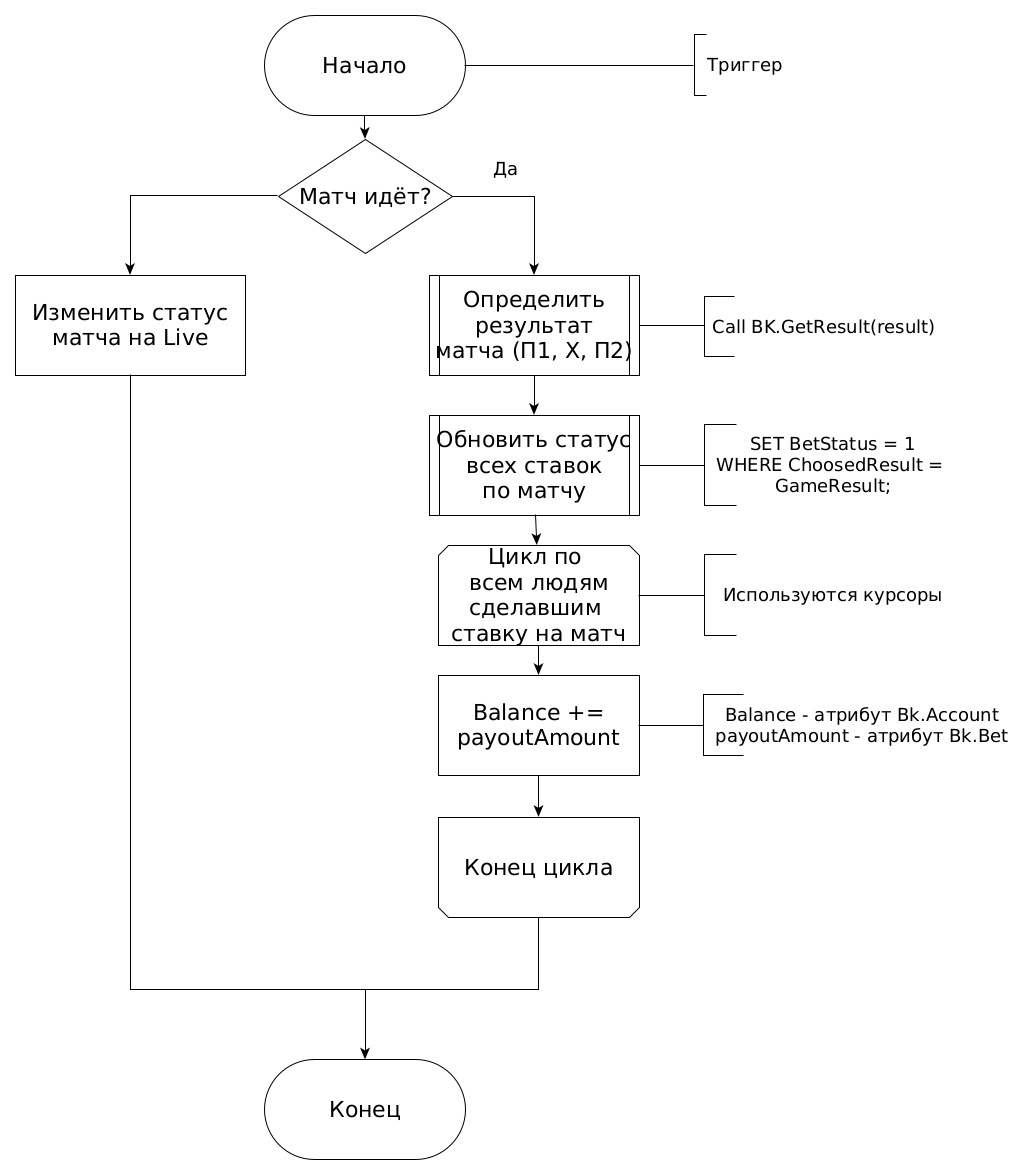
\includegraphics[height=18cm, width=\linewidth]{inc/updateFlow.png}
	\end{center}
	\captionsetup{justification=centering, labelsep=defffis}
	\caption{Схема алгоритма обновления состояния матча}
	\label{fig::update}
\end{figure}
\FloatBarrier
